% =====================================================================
\chapter{Implementation and Experimental Results on Hardware}
\label{ch:impl}
\thispagestyle{plain}
% =====================================================================

\section{Introduction}

A precoder or controller that is accurate in simulation is only useful if it meets the real-time budget of the O-DU. This chapter describes the implementation side of the project: the hand-optimised C/AVX-512/OpenMP kernel that computes the whole RZF precoder of Eq.~\eqref{eq:rzf} for 273 PRBs in a fraction of the 0.5~ms slot (Sections~\ref{sec:hw-platform}--\ref{sec:hw-results}), and the software framework used for every experiment of this report (Section~\ref{sec:sw}).

\section{Hardware Platform}
\label{sec:hw-platform}

All timing measurements were made on a 4-core Intel Xeon server CPU with AVX-512 support, the class of general-purpose processor used in software-defined, cloud-native O-DU deployments. Kernels were compiled with GCC and timed with \texttt{rdtsc} cycle counters for per-stage profiling and with wall-clock time (median of 40 runs) for end-to-end results. The data type is single-precision complex (\texttt{complex64}), as used in O-DU baseband processing; accuracy is always checked against a float64 reference.

\section{Design of the Fused RZF Precoder Kernel}
\label{sec:hw-kernel}

The kernel (\texttt{kernels/cmat\_kernels.c}, Python binding \texttt{cmatinv/fastkernels.py}) is a batched complex64 implementation of $G = HH^H + \alpha I$, $G^{-1}$ and $W = H^H G^{-1}$ for all PRBs of a slot. Figure~\ref{fig:kernel} shows its dataflow. The key design decisions are:

\begin{itemize}
  \item \textbf{One fused pass per PRB.} $H$ is loaded once; Gram, inverse, $W^T$ and power scaling are computed back-to-back on stack and L1-resident buffers, with no DRAM intermediates.
  \item \textbf{Hermitian symmetry.} Only the lower triangle of the Gram matrix is computed.
  \item \textbf{Split real/imaginary planes} (structure of arrays), so that complex arithmetic vectorises cleanly.
  \item \textbf{In-place Gauss--Jordan sweep inverse.} $K$ rank-1 updates on contiguous, fully vectorised rows, without square-root or division chains; no pivoting is needed because $G \succ 0$ (a Cholesky path is kept behind \texttt{-DUSE\_CHOL}).
  \item \textbf{Register-blocked weight formation} $W = H^H X$, with output layout $W^T[S,K,M]$.
  \item \textbf{AVX-512 code generation} (\texttt{-mprefer-vector-width=512}; GCC defaults to 256-bit vectors).
  \item \textbf{OpenMP} \texttt{parallel for} across the 273 PRBs and \texttt{omp simd} inner loops.
  \item \textbf{Fused Newton step} for the RMT-WS warm start, which returns the exact residual $\|I - GX\|_F/\sqrt K$ at no extra cost.
\end{itemize}

\begin{figure}[H]
\centering
\begin{tikzpicture}[font=\footnotesize,>=Stealth,
   s/.style={draw,rounded corners,align=center,minimum height=1.05cm,text width=2.25cm,fill=soft},
   g/.style={s,fill=good!15}]
  \node[s,fill=iitblue!12] (h) {Load $H$\\(re/im planes)};
  \node[s,right=0.45cm of h] (gram) {Gram\\lower triangle\\$HH^H + \alpha I$};
  \node[g,right=0.45cm of gram] (inv) {GJ sweep inverse\\or fused\\Newton step};
  \node[s,right=0.45cm of inv] (w) {$W^T = (H^H G^{-1})^T$\\register-blocked};
  \node[s,right=0.45cm of w,fill=orange!15] (sc) {Power\\scaling\\$\to$ output};
  \draw[->,thick] (h) -- (gram);
  \draw[->,thick] (gram) -- (inv);
  \draw[->,thick] (inv) -- (w);
  \draw[->,thick] (w) -- (sc);
  \node[draw,dashed,rounded corners,fit=(h)(gram)(inv)(w)(sc),inner sep=7pt,label={[font=\footnotesize]below:one PRB, L1-resident, AVX-512 \texttt{omp simd} \qquad $\times$ 273 PRBs in parallel (OpenMP)}] {};
\end{tikzpicture}
\caption{Dataflow of the fused RZF precoder kernel for one PRB; PRBs are processed in parallel across cores.}
\label{fig:kernel}
\end{figure}

The inner loop of the sweep inverse illustrates the style of the kernel: one rank-1 update of all rows except the pivot row, written so that the compiler emits fused multiply-add AVX-512 instructions on the split real and imaginary planes.

\begin{lstlisting}
// inner loop of the in-place Gauss-Jordan sweep inverse (pivot k)
for (int i = 0; i < K; i++) {
  if (i == k) continue;
  float fr = ckr[i]*piv, fi = cki[i]*piv;
  float *ar = xr + i*K, *ai = xi + i*K;
  #pragma omp simd
  for (int j = 0; j < K; j++) {
    ar[j] -= fr*rkr[j] - fi*rki[j];
    ai[j] -= fr*rki[j] + fi*rkr[j];
  }
  ar[k] = -fr; ai[k] = -fi;
}
\end{lstlisting}

The kernel is built with
\begin{lstlisting}[language=bash]
gcc -O3 -march=native -fopenmp -ffast-math \
    -mprefer-vector-width=512 -shared -fPIC cmat_kernels.c -o libcmat.so -lm
\end{lstlisting}

\section{Profiling-Driven Optimisation}
\label{sec:hw-opt}

The kernel was optimised step by step, guided by per-stage cycle counts ($K=16$, $M=64$, one thread):
\begin{enumerate}
  \item \textbf{Fusion and Hermitian symmetry}: the Gram matrix is formed on the lower triangle only, inside the per-PRB pass.
  \item \textbf{Register-blocked weight formation} $W = H^H X$ with output $W^T[S,K,M]$: from 0.81 to \textbf{0.42~ms} per slot.
  \item \textbf{Gauss--Jordan sweep instead of Cholesky}: the inverse drops from 6.4k to \textbf{2.9k cycles} per PRB at $K=16$, and from 21k to 11k cycles at $K=32$.
  \item \textbf{AVX-512 code generation}: 1.3--1.5$\times$ faster on one thread and 2$\times$ on four threads.
  \item A 4-column blocked Gram variant was measured and reverted because it was slower.
\end{enumerate}
After tuning, weight formation takes 44--58\,\% of the cycles at about 30 flops/cycle (about half of the AVX-512 peak), the Gram matrix 20--24\,\% at about 28 flops/cycle, and the inverse the rest.

\section{Experimental Results}
\label{sec:hw-results}

\subsection{Whole precoder per slot}

Table~\ref{tab:hw-pipeline} and Figure~\ref{fig:hw-pipeline} report the time to compute the complete precoder (Gram, inverse and weights) for all 273 PRBs of a slot. \textbf{The fused kernel is 10--15$\times$ faster than numpy + LAPACK.} For $K = 16$ users and $M = 64$ antennas it takes 0.226~ms, less than half of the 0.5~ms slot, where numpy + LAPACK needs 3.21~ms, six times the slot. With the kernel, $K = 8$ and $K = 16$ at $M = 64$, and $K = 16$ at $M = 128$, \textbf{fit the slot for the entire precoder}. None of these configurations did before. Thread scaling is near-linear: 0.92, 0.45 and 0.23~ms on 1, 2 and 4 threads.

\begin{table}[H]
\caption{Whole-precoder time per slot (273 PRBs, complex64, 4-core AVX-512 Xeon, median of 40 runs).}
\label{tab:hw-pipeline}
\centering
\begin{tabular}{lcccc}
\toprule
$K$, $M$ & numpy + LAPACK & Our kernel, 1 thread & \textbf{Our kernel, 4 threads} & Speed-up \\
\midrule
8, 64 & 1.08~ms & 0.268~ms & \textbf{0.070~ms} & 15$\times$ \\
\ours 16, 64 & 3.21~ms & 0.917~ms & \textbf{0.226~ms} & \textbf{14$\times$} \\
32, 64 & 12.2~ms & 3.75~ms & 0.97~ms & 12.5$\times$ \\
16, 128 & 4.71~ms & 1.61~ms & \textbf{0.41~ms} & 11.6$\times$ \\
32, 128 & 16.3~ms & 6.43~ms & 1.60~ms & 10$\times$ \\
\bottomrule
\end{tabular}
\end{table}

\begin{figure}[H]
\centering
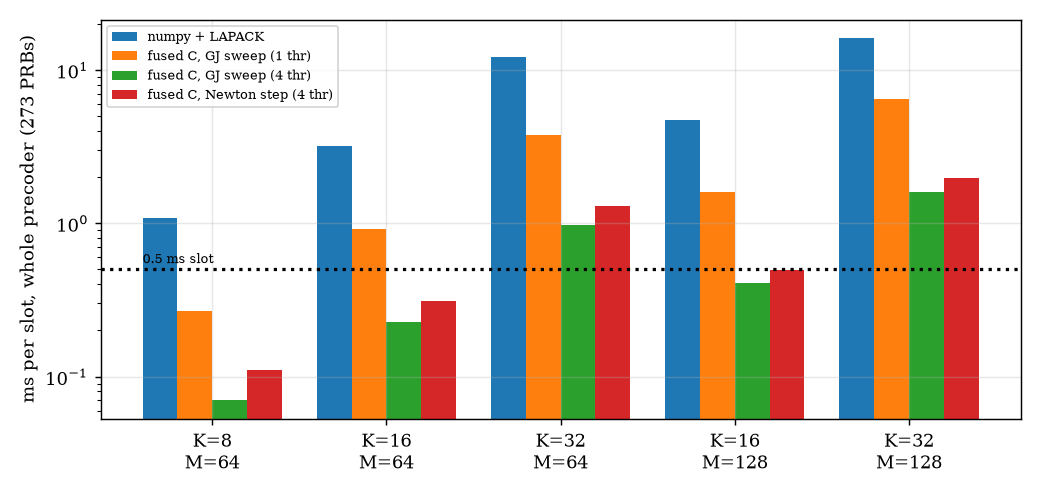
\includegraphics[width=\textwidth]{exp17_pipeline_kernel.png}
\caption{Whole-precoder time per slot; the fused kernels run below the 0.5~ms slot line for $K \le 16$, while numpy + LAPACK never does.}
\label{fig:hw-pipeline}
\end{figure}

\subsection{Inverse kernels}

Figure~\ref{fig:hw-inv} isolates the inverse. The C kernels are an order of magnitude faster than numpy/LAPACK, and the \textbf{fused Newton--Schulz step of RMT-WS is the fastest inverse for $K \le 16$} (0.115~ms per slot at $K=16$, against 0.124~ms for a tuned C Cholesky inverse and 1.6~ms for LAPACK). This is the per-slot warm-start update of Chapter~\ref{ch:parta-methods} running at hardware speed.

\begin{figure}[H]
\centering
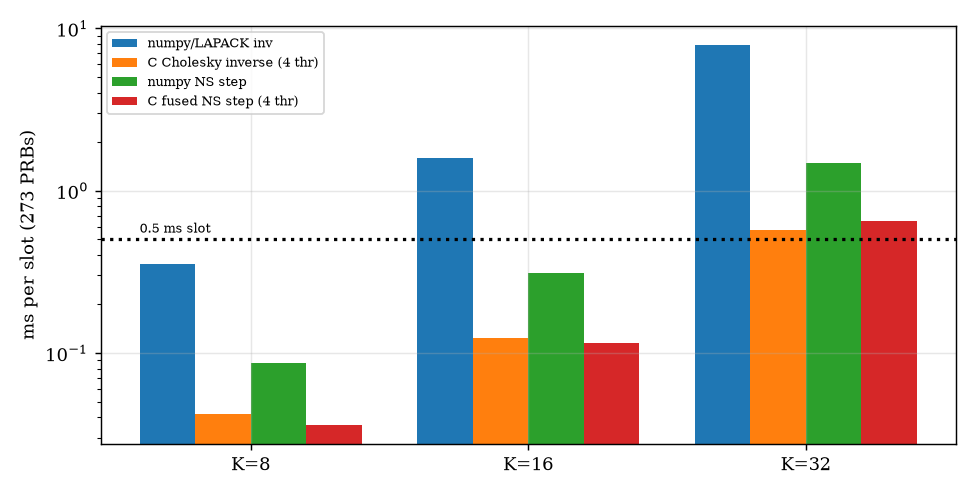
\includegraphics[width=0.85\textwidth]{exp15_kernel_bench.png}
\caption{Inverse-only time per slot (273 PRBs): numpy/LAPACK, tuned C Cholesky, numpy Newton--Schulz step and our fused C Newton--Schulz step (4 threads).}
\label{fig:hw-inv}
\end{figure}

\subsection{Accuracy}

The complex64 kernel reproduces the float64 exact precoder with a sum-rate loss of about $10^{-6}\,\%$ or less in every tested configuration ($K=16$ at 10 and 30~dB, an ill-conditioned 3$^\circ$-spread channel at 25~dB, $K=32$ at 20~dB and $K=16$, $M=128$ at 30~dB). The speed-up therefore comes at no cost in link performance.

\section{Software Framework and Reproducibility}
\label{sec:sw}

All results of this report are produced by an open, fully reproducible Python/C code base (Table~\ref{tab:repo}). The Part~B simulator is slot-accurate: it generates the three traffic families, applies the stale observations and the held budgets, runs FIFO queues with deadline drops for every cell and records every metric. Every number in our papers is generated as a macro from the result CSV files, so text and data cannot diverge.

\begin{table}[H]
\caption{Structure of the project repository.}
\label{tab:repo}
\centering\small
\begin{tabularx}{\textwidth}{>{\ttfamily}p{4.4cm}X}
\toprule
\normalfont Module & Content \\
\midrule
matinv\_bench/ & inversion benchmark, InverseNet-MLP/NS/Ultra \\
cmatinv/, experiments\_v2/ & complex inversion, RMT-WS, 38.901 channels, Experiments 5--18 \\
kernels/ & fused C/AVX-512/OpenMP precoder kernel \\
experiments/ & Part~A Experiments 1--4, extended Part~B pipeline \\
fhlm/ & Part~B simulator, traffic families S, G, M, forecasters, 19+ controllers, theory, figures, tables \\
fhlm/transformer.py, decision\_focused.py & B2: LCQT, Bayesian mixture, differentiable KKT layer \\
fhlm/hybrid.py & B3: back-pressure newsvendor and equal-budget CEM search \\
tests/ & 46 unit tests: capacity in every slot, no future leakage, bound validity, KKT-layer gradients, policy containment \\
results/ & all CSV files, logs and figures \\
\bottomrule
\end{tabularx}
\end{table}

\paragraph{Verification.} The unit tests check, among other properties, that the link capacity is respected in every slot, that no feature uses future data, that the deadline-feasible rate is tight, that the theoretical bounds hold, that the differentiable KKT layer matches the numpy allocator to $10^{-6}$ with correct gradients, and that BPN reproduces predictive MaxWeight and the CEM policy exactly with the corresponding parameters.

\section{Discussion and Analysis}

This chapter discussed the hardware results of the project. The fused C/AVX-512/OpenMP kernel turns the RZF precoder from a computation that is six times too slow for the slot into one that uses less than half of it, with float64-level accuracy. This is what makes per-slot RU-side precoding, with its 72\,\% fronthaul saving, practical on a general-purpose CPU O-DU. On the Part~B side, every controller runs well within its 10~ms decision interval in Python (3.5~ms for the KKT rule with GBM, 2.2--3.5~ms for BPN), and the fully tested, reproducible framework makes every result of this report traceable to its data.
